%!TEX root = ../diss.tex
\tikzstyle{element}=[rectangle, thick,
                     inner sep=0.1cm, rounded corners]
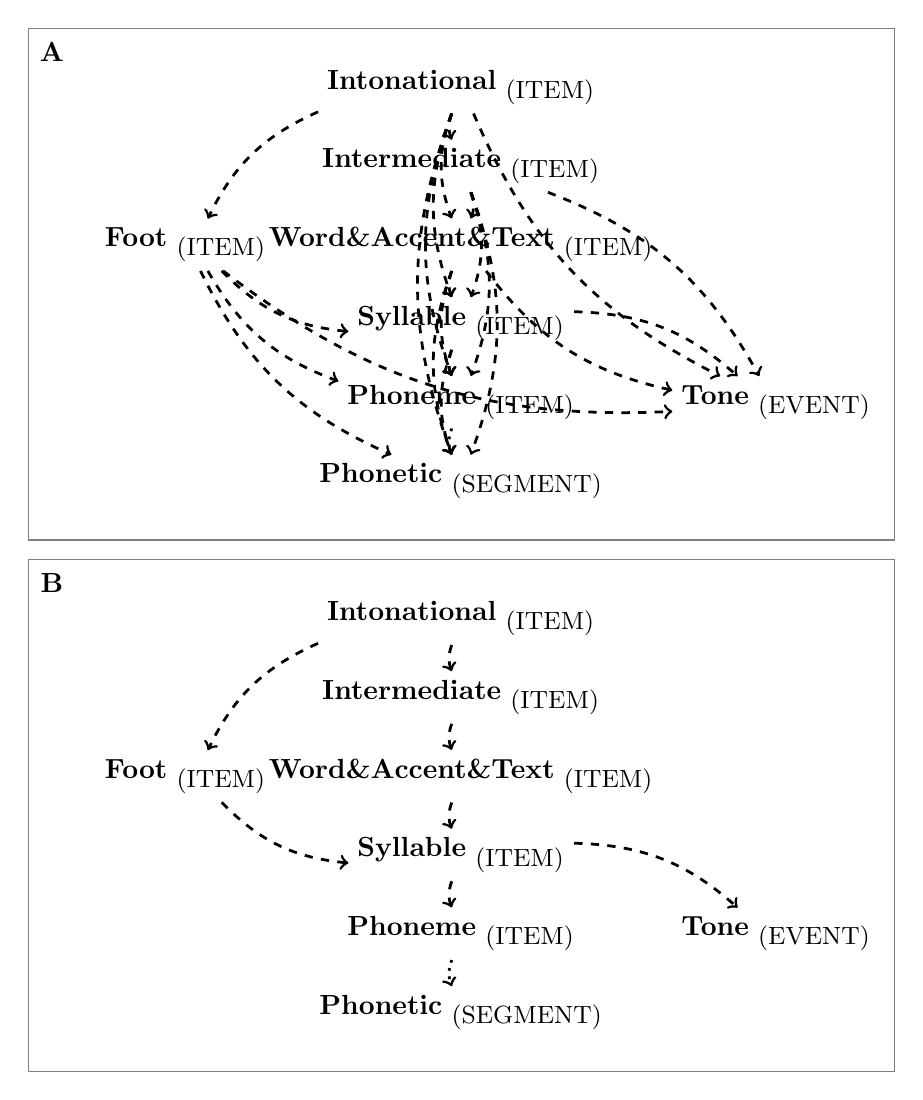
\begin{tikzpicture}
%%%%%%%%%%%%%%%%%%%%%%%%%%%%%%
% nodes

% a
\draw[gray] (-5.5, 11.5) rectangle (5.5, 5);
\node (a) at (-5.2, 11.2){\textbf{A}};

\node (into_a) at (0, 10.75) [element] {\textbf{Intonational} \textsubscript{\small{(ITEM)}}};

\node (interm_a) at (0, 9.75) [element] {\textbf{Intermediate} \textsubscript{\small{(ITEM)}}};

\node (word_a) at (0, 8.75) [element] {\textbf{Word\&Accent\&Text} \textsubscript{\small{(ITEM)}}};

\node (foot_a) at (-3.5, 8.75) [element] {\textbf{Foot} \textsubscript{\small{(ITEM)}}};

\node (syl_a) at (0, 7.75) [element] {\textbf{Syllable} \textsubscript{\small{(ITEM)}}};

\node (phoneme_a) at (0, 6.75) [element] {\textbf{Phoneme} \textsubscript{\small{(ITEM)}}};

\node (tone_a) at (4, 6.75) [element] {\textbf{Tone} \textsubscript{\small{(EVENT)}}};

\node (phonetic_a) at (0, 5.75) [element] {\textbf{Phonetic} \textsubscript{\small{(SEGMENT)}}};


% b
\draw[gray] (-5.5, 4.75) rectangle (5.5, -1.75);
\node (b) at (-5.2, 4.45){\textbf{B}};

\node (into_b) at (0, 4) [element] {\textbf{Intonational} \textsubscript{\small{(ITEM)}}};

\node (interm_b) at (0, 3) [element] {\textbf{Intermediate} \textsubscript{\small{(ITEM)}}};

\node (word_b) at (0, 2) [element] {\textbf{Word\&Accent\&Text} \textsubscript{\small{(ITEM)}}};

\node (foot_b) at (-3.5, 2) [element] {\textbf{Foot} \textsubscript{\small{(ITEM)}}};


\node (syl_b) at (0, 1) [element] {\textbf{Syllable} \textsubscript{\small{(ITEM)}}};

\node (phoneme_b) at (0, 0) [element] {\textbf{Phoneme} \textsubscript{\small{(ITEM)}}};

\node (tone_b) at (4, 0) [element] {\textbf{Tone} \textsubscript{\small{(EVENT)}}};

\node (phonetic_b) at (0, -1) [element] {\textbf{Phonetic} \textsubscript{\small{(SEGMENT)}}};


%%%%%%%%%%%%%%%%%%%%%%%%%%%%%%
% links

% a
\draw [->, line width=1, dashed] (into_a) to [bend right=20] (interm_a);
\draw [->, line width=1, dashed] (into_a) to [bend right=20] (foot_a);
\draw [->, line width=1, dashed] (into_a) to [bend right=20] (word_a);
\draw [->, line width=1, dashed] (into_a) to [bend right=20] (syl_a);
\draw [->, line width=1, dashed] (into_a) to [bend right=20] (phoneme_a);
\draw [->, line width=1, dashed] (into_a) to [bend right=20] (tone_a);
\draw [->, line width=1, dashed] (into_a) to [bend right=20] (phonetic_a);

\draw [->, line width=1, dashed] (interm_a) to [bend left=20] (word_a);
\draw [->, line width=1, dashed] (interm_a) to [bend left=20] (syl_a);
\draw [->, line width=1, dashed] (interm_a) to [bend left=20] (phoneme_a);
\draw [->, line width=1, dashed] (interm_a) to [bend left=20] (tone_a);
\draw [->, line width=1, dashed] (interm_a) to [bend left=20] (phonetic_a);

\draw [->, line width=1, dashed] (word_a) to [bend right=20] (syl_a);
\draw [->, line width=1, dashed] (word_a) to [bend right=20] (phoneme_a);
\draw [->, line width=1, dashed] (word_a) to [bend right=20] (tone_a);
\draw [->, line width=1, dashed] (word_a) to [bend right=20] (phonetic_a);

\draw [->, line width=1, dashed] (foot_a) to [bend right=20] (syl_a);
\draw [->, line width=1, dashed] (foot_a) to [bend right=20] (phoneme_a);
\draw [->, line width=1, dashed] (foot_a) to [bend right=20] (tone_a);
\draw [->, line width=1, dashed] (foot_a) to [bend right=20] (phonetic_a);

\draw [->, line width=1, dashed] (syl_a) to [bend right=20] (phoneme_a);
\draw [->, line width=1, dashed] (syl_a) to [bend right=20] (phonetic_a);

\draw [->, line width=1, dashed] (syl_a) to [bend left=20] (tone_a);

\draw [->, line width=1, dotted] (phoneme_a) to [bend right=20] (phonetic_a);

% b
\draw [->, line width=1, dashed] (into_b) to [bend right=20] (interm_b);

\draw [->, line width=1, dashed] (into_b) to [bend right=20] (foot_b);

\draw [->, line width=1, dashed] (interm_b) to [bend right=20] (word_b);

\draw [->, line width=1, dashed] (word_b) to [bend right=20] (syl_b);

\draw [->, line width=1, dashed] (foot_b) to [bend right=20] (syl_b);

\draw [->, line width=1, dashed] (syl_b) to [bend right=20] (phoneme_b);

\draw [->, line width=1, dashed] (syl_b) to [bend left=20] (tone_b);

\draw [->, line width=1, dotted] (phoneme_b) to [bend right=20] (phonetic_b);


\end{tikzpicture}
